% Add this to your preamble (in your main document file, not this file)
% \newfontfamily\greekfonttt[Script=Greek]{DejaVu Sans Mono}

\section{Προγράματισμος των μικροελεκτών}

\cite{Ahmed2019}

\subsection{Εργαλία που χρησιμοποιήθηκαν για την ανάπτυξη του λογισμικού}
Για την ανάπτυξη του λογισμικου του μικροελεκτή, η ανάπτυξη του κώδικα γράφτηκε στον Visual Studio code,χρησιμοποιώντας σαν extention το Platform IO IDE και το Arduino framework. 


\subsubsection{Visual studio code και Platform IO}

Το Visual Studio Code είναι ένα δωρεάν στην χρήση, χαμηλών απαιτήσεων πρόγραμμα επεξεργασίας πηγαίου κώδικα (source-code editor),το οποίο μπορεί να λειτουργήσει σε πολλαπλά λειτουργικά συστήματα,στα Windows,macOS, Linux και Raspberry Pi OS,ανεπτυγμένo από την Microsoft και έχοντας εκδοθεί το 2015. 
Είναι λογισμικό αναπτυγμένο με το Electro framework και Node js, ανοιχτού κώδικα και διανέμεται υπό την άδεια MIT (MIT License) ,το οποίο κυκλοφόρησε το 2015\cite{TechCrunch2015},\cite{InfoWorld2022}.

Αποτελεί την πιο δημοφιλή επιλογή ολοκληρωμένου περιβάλλοντος ανάπτυξης (Integrated development environment,IDE) εδώ και πολλαπλά χρόνια \cite{StackOverflow2025}.Προσφέρει δυνατότητες όπως είναι οι βασικές λειτουργίας προγράμματος επεξεργασία πηγαίου κώδικα, όπως είναι επισύμανση κώδικα και αποσπάσματα κώδικα (code snippets),ενσωματωμένο terminal,την έξυπνη αυτοσυμπλήρωση κώδικα που προσφέρει σαν εργαλείο το IntelliSense,ενσωματομένο Debugging και version control, όπως και μία πολύ μεγάλη πληθώρα επεκτάσεων (extentions), όπου μπορούν να προσθέσουν έξτρα λειτουργικότητες,υποστήριξη για διάφορες γλώσσες προγραμματισμού, μέχρι και εξειδικευμένα IDE για την ανάπτυξη λογισμικού. Τα extention αυτά μεταμορφώνουν το Visual studio code από ένα code editor σε ένα πλήρες IDE για την ανάπτυξη λογισμικού \cite{HOSTINGER2025}.


\begin{figure}[!htbp]
    \centering
    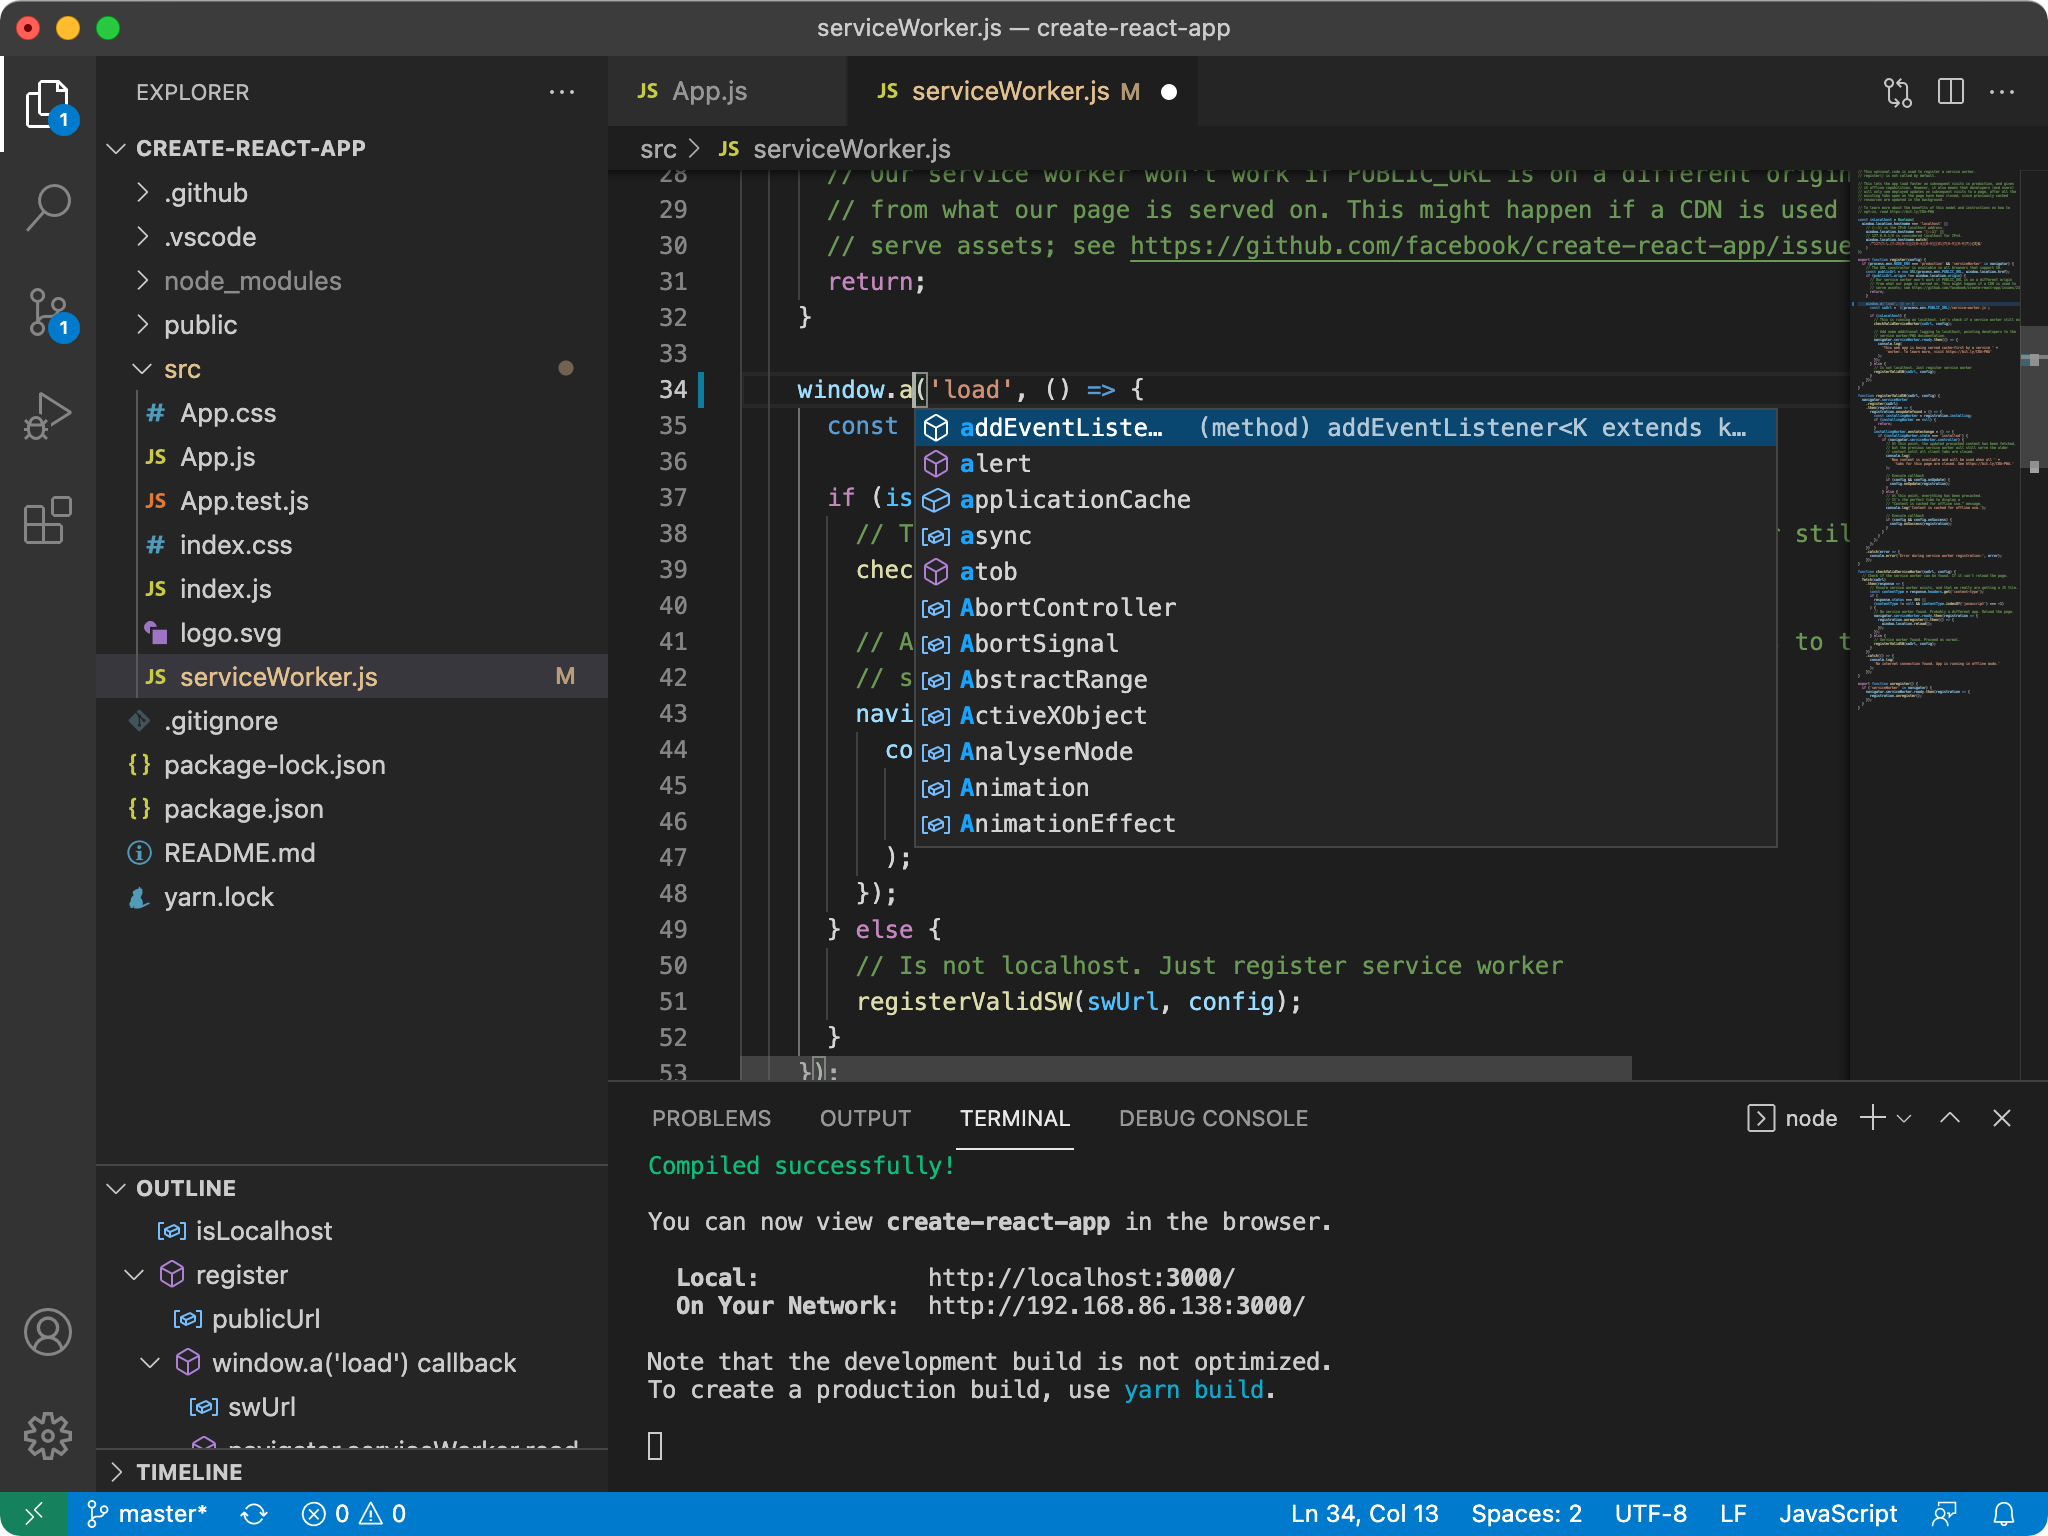
\includegraphics[width=0.8\textwidth]{εικόνες/Εργαλία που χρησιμοποιήθηκαν για την ανάπτυξη του λογισμικού/εικόνα τυπικού visual studio workload.png}
    \caption{Το περιβάλλον του visual studio code \cite{GitHubVSCODE}}
    \label{fig:PLATFORM IO HOME PAGE}
\end{figure}

\FloatBarrier 

Ένα τέτοιο extention είναι το Platform IO IDE, το οποίο κάνει πολύ εύκολη την ανάπτυξη λογισμικού για μια πληθώρα διαφορετικών μικροελεκτών,πλακετών ανάπτυξης (development broad) και γενικότερα ενσωματομένων συστημάτων. Διαχειρίζεται τις αναγκαίες εξαρτήσεις βιβλιοθηκών,πακέτων και αρχείων,όπως και τα αναγκαία toolchain και compilers που χρειάζεται η κάθε ενσωματομένη πλατφόρμα,πλακέτα ανάπτυξης και framework που χρησιμοποιείται,όπως είναι το arduino framework και ανεβάζει το λογισμικό στην ανάλογη φυσική πλακέτα ανάπτυξης.
Επίσης,προσφέρει πολλά εργαλεία για ευκολότερο debugging,unit testing,αυτόματη ανάλυση στατικού κώδικα και ανάπτυξη από απόσταση \cite{PlatformIOINTRO}. To Platform IO IDE έχει σαν βασικά μέλη λειτουργίας το PlatformIO Core,που συντελούνται οι λειτουργίες του Platform IO IDE,και το PlatformIO Home,που αποτελεί την διαπεφή με τον χρήστη (User interface,UI).Το Platform IO Core έχει προγραμματιστεί εξ' ολοκλήρου με Python και το PlatformIO υλοποιήται με το Modern UI Toolkit της PlatformIO Labs





Για την επιλογή των διαφώρων διεργασιών που χρειάζεται να τελεσθούν για να τρέξει το λογισμικό που προγραμματίζει ο χρήστης σε ένα ή πολλά συγκεκριμένα ενσωματομένα συστήμα, χρησιμοποείται στο υψηλότερο φάκελο (root directory) του κάθε project   να αρχείο διαμόρφωσης (configuration file),που ονομάζεται \textbf{platformio.ini}. 

Στο συγκεκριμένο αρχείο μπορούν να οριστούν ρυθμίσεις που να αφορούν την λειτουργία όλου του project και να αλλάζουν τις προεπιλεγμένες ρυθμίσεις του project, κάτω από την κατηγορία  \textbf{[platformio]}.
Επιπλέον μπορούν να δημιουργηθούν πολλές διαφορετικές ομάδες ρυθμίσεων στο ίδιο το project, οι οποίες μπορεί να αφορούν ρυθμίσεις για ενσωματωμένες συσκευές με διαφωρετικά χαρακτηριστικά, όπως διαφορετικο development board και αρχιτεκτονική μικροελεγεκτή (platform),για τον ίδιο κώδικα που έχει κατασκευαστεί από το χρήστη.
Αλλά  μπορούν να υπάρχουν και ξεχωριστές ομάδες με διαφορετικές ρυθμίσεις για την ίδιο την ενσωματωμένη συσκεή ,ή συσκευές με την ίδια πλακέτα ανάπτυξης,με χαρακτηριστικό παράδειγμα τις κατασκευαστικές ρυθμίσεις, αναφερόμενες στην τεκμιρίωση (documentation) του PlatformIO και εώς \textbf{build\_type}  και οι 3 επιλεγμένες ρυθμίσεις είναι το \textbf{release,test,debug}.Όλες οι ομάδες αναφέρονται έως  \textbf{[env:Όνομα]},καθώς οι διαφορετικές ομάδες είναι διαφορετικά αυτόνομα περιβάλλοντα  \cite{PlatformIOCONFIG}.


Οι ρυθμίσεις που χρησιμοποιήθηκαν για το project που υλοποιήθηκε για προγραμματισμό των αισθητήρων ήταν αυτά που αναφέρονται στην \autoref{fig:PLATFORM IO CONFIG}.H έκδοση του PlatformIO Core που χρησιμοποιήθηκε είναι η 6.1.18.

\begin{figure}[!htbp]
    \centering
    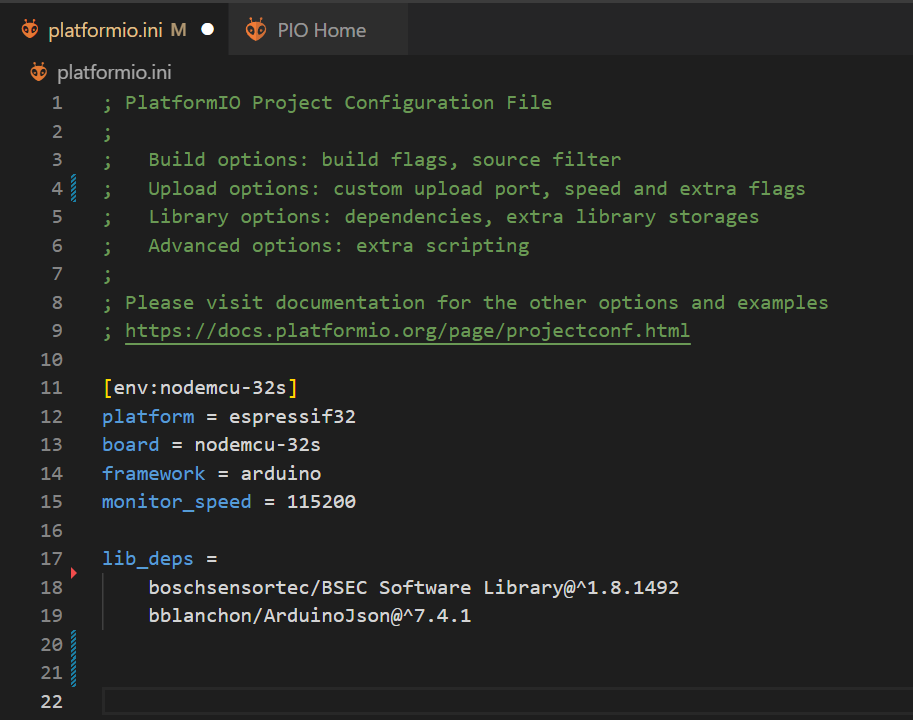
\includegraphics[width=0.8\textwidth]{εικόνες/Εργαλία που χρησιμοποιήθηκαν για την ανάπτυξη του λογισμικού/config.png}
    \caption{Configuration που χρησιμοποιήθηκαν για το project}
    \label{fig:PLATFORM IO CONFIG}
\end{figure}


\FloatBarrier 

Το \fbox{env:nodemcu},είναι το μοναδικό περιβάλλον που έχουμε στο project,καθώς χρησιμοποιοήθηκαν και για τις τρεις συσκεύες που αναπτύχθηκαν ο ίδιος μικροελεκτής και η ίδια πλακέτα ανάπτυξης.
Η πλατφόρμα \fbox{platform = espressif32} και  η πλακέτα \fbox{board = nodemcu-32s} είναι αντίστοιχα η αρχιτεκτονική esp32 και η πλακέτα nodemcu-32s που χρησιμοποιήσαμε για την κατασκευή των μικροελεκτών και μιλήσαμε παραπάνω. 
Το monitoring speed εκφράζεται σε baud rate,με baud rate ο ρυθμός με τον οποίο μεταφέρονται οι πληροφορίες σε ένα κανάλι επικοινωνίας \url{https://randomnerdtutorials.com/esp32-uart-communication-serial-arduino/}. Στην περίπτωση μας,μας επιτρέπει να στέλνονται μηνύματα και να λαμβάνονται μηνύματα μέσω καλωδίου από τον μικροελεκτή στον υπολογιστή μας,μέσω καλωδίου, και να διαβάζονται στον Serial Monitor του IDE μας. Το baud rate για τους esp32 microcontroller είναι 115200.

Το \fbox{framework = arduino} μας δίνει την δυνατότητα να "τυλιξούμε" (wrapping) το esp-idf με το API του Arduino,οπότε να μπορούμε να προγραμματίσουμε τους esp32 με τις συναρτήσεις και την δομή της γλώσσας προγραμματισμού του Arduino  (Application Programming Interface). Αυτό το wrapper για το esp-idf ονομάζεται Arduino Core \cite{EspressifArduinoCore},με την έκδοση που χρησιμοποιήθηκε να είναι η 3.20017.0. 
Τo arduino έχει προγραμματιστεί με c++,αλλά μπορεί να χρησιμοποιήθει και με c  στον προγραμματισμό και το esp-idf έχει προγραμματιστεί σε c αλλά μπορεί να υποστηρίξει και c++ \url{https://docs.espressif.com/projects/esp-idf/en/stable/esp32/api-guides/cplusplus.html}.

\subsubsection{Γλώσσα προγραμματισμού Arduino}

Το Arduino API ,και γενικά τα προιόντα της Arduino (υλικό και λογισμικό) ,αποτελούν την πιο δημοφιλή και προσιτή επιλογή στον τομέα των ενσωματωμένων συστημάτων.
Η δομή του προσφέρει εύκολο και γρήγορο προγραμματισμό μικροελεκτών,ακόμα και σε άτομα που δεν έχουν εξιδικευμένη γνώση στα ενσωμετομένα συστήματα. Ένα άλλο μεγάλο της θετικό είναι η μεγάλη κοινότητα που υπάρχει γύρω από τους Arduino μικροελεκτές και λογισμικό, κάνοντας την αναζήτηση γνώσεων και την εύρεση σχετικών με κάποιο ζήτημα βιβλιοθηκών πολύ πιο εύκολο σε σχέση με την esp-idf, που έχει μια πιο μικρή και εξιδεικευμένη κοινότητα.
Η λέξη arduino  μπορεί να χρησιμοποιήθει εναλλάξ για να αναφερθεί στους μικροελεκτές Arduino,στο Arduino IDE και στην προγραμματιστική γλώσσα Arduino,που χρησιμοποιείται για τον προγραμματισμό μικροελεκτών Arduino και στο Arduino Core.

Στη \textit{}{setup()} και στην \textit{loop()} , όπου η πρώτη συνάρτηση εκτελείται την στιγμή που ξεκινάει το πρόγραμμα, ή sketch όπως το αποκαλεί το arduino documentation, να λειτουργεί,που συνήθως αυτό συμβαίνει όταν αποκτά πρόσβαση σε ρεύμα ή πατιέται το κουμπί reset της πλακέτας του μικροελεκτή. Στην \textit{setup()} είναι που αρχικοποιούνται οι μεταβλητές,οι βιβλιοθήκες και τα pin εισόδου και εξόδου. Μετά την εκτέλεση της \textit{setup()},η συνάρτηση \textit{loop()} εκτελείται συνεχόμενα,για όσο ο μικροελεκτής είναι ενεργός.Το \textit{loop()} εμπεριέχει το βασικό κομμάτι του κώδικα.\url{https://docs.arduino.cc/language-reference/#structure} 

Η μεγάλη διαφορά μεταξύ της Arduino γλώσσας και το esp-idf είναι ότι το Arduino μπορεί να διαχειριστεί μόνο ένα νήμα (single thread) εκτέλεσης διεργασίας και διαχειρίζεται τον κώδικα σειριακά. 
Αντίθετα,επειδή το esp-idf βασίζεται στο FreeRTOS,μπορεί να υπάρχουν πολλά νήματα (multi-threaded) εκτέλεσης διεργασιών παράλληλα.
Υπάρχουν δύο δυνατότητες που προσφέρει η Arduino γλώσσα που μπορεί να μυμιθεί αυτή την λειτουργια
Δίνεται η δυνατότητα να υπάρξει διακοπή (interrupt) της λειτουργίας της συνάρτησης \textit{loop()} και εκτέλεση μίας συνάρτησης που έχει οριστεί σαν απάντηση στην διακοπη αυτή όταν ένα pin φτάνει σε μια συγκεκριμένη κατάσταση \url{https://docs.arduino.cc/language-reference/en/functions/external-interrupts/attachInterrupt/},ωστέ να μπορεί να αντιδράσει ο μικροελεκτής σε συγκεκριμένα γεγονότα (events) ή χρονιστές (timers). 
Όμως η συνάρτηση που εκτελείται ως διακοπή πρέπει να είναι μικρή σε έκταση για να μην μπλοκάρει ενέργειες που πρέπει να γίνουν από άλλες διακοπές ή το κανονικό κομμάτι του κώδικα που εκτελείται στην \textit{loop}

Ακόμα,με την χρήση της συνάρτησης \textit{millis()},που μετράει τα πόσα milliseconds έχουν περάσει από την έναρξη λειτουργίας του μικροελεκτή \url{https://docs.arduino.cc/language-reference/en/functions/time/millis/} μπορείς να πετύχεις να εκτελέσεις διεργασίες με βάση το χρονικό διάστημα που έχει περάσει,χωρίς να χρησιμοποιηθεί διακοπή, με το να συγκρίνεις τα milliseconds που έχουν μετρηθεί την δεδομένη χρονική στιγμή σε μία παλιότερη χρονική στιγμή που χρησιμοποιήθηκε το millis().Παρόλα αυτά, συνεχίζει η γλώσσα arduino να μπορεί να τρέξει μόνο σειριακά.

Η δυνατότητα multi-threaded που προσφέρει το esp-idf,η καλύτερη χρήση των δύο επεξαργαστών του esp32 και μη ανάγκη του να τρέξουν πολλες διεργασίες κρυφά από τον χρήστη για να μπορέσει να λειτουργήσει το arduino core με τόσο εύκολο για τον χρήστη τρόπο κάνει το esp-idf την καλύτερη επιλογή για καλύτερη αποδοτικότητα \url{https://www.espboards.dev/blog/esp-idf-vs-arduino-core/}.
Ωστόσο,στο project που υλοποιήθηκε, δεν χρειάστηκαν οι δυνατότητες του esp-idf,μολονότι η απλότητα της γλώσσας arduino αποτέλεσε εμπόδιο για τις πολλαπλε΄ς





